% Chapter ?

\clearpage
Un punteo de los cambios más importantes respecto a la versión anterior del informe:

Section 3.1:
\begin{itemize}
\vspace{-10pt}
\item Agregué la Definition 3.1.3. Eso me permitió acortar las definiciones de CR y RD, ya que en la versión anterior del informe después de cada ecuación ponía explícitamente qué significaba cada uno de los tamaños $|c(z,f)|$, etc.

\item En la Section 3.2 los experimentos consideran siempre todos los archivos del dataset (nunca consideran un archivo en particular), pero en la Section 3.3 consideran archivos particulares (porque se toma la ventana óptima para cada archivo). En la versión anterior del informe las definiciones de CR y RD siempre eran función de un archivo particular, que en realidad no era del todo correcto para la forma en que se aplican en la Section 3.2, pero como todavía no había escrito la Section 3.3, se podía considerar un abuso de notación (i.e. podía considerar al dataset un archivo creado a partir de todos los archivos concatenados). Pero al escribir la Section 3.3 me pareció que tenía que pulir un poco más las definiciones de CR y RD para cada caso (archivo particular vs. dataset). Entonces al final de la Section 3.1 agregué unas definiciones nuevas en ese sentido. 
\end{itemize}

Section 3.2:
\begin{itemize}
\vspace{-10pt}
\item No sé si el primer párrafo / definición quedan del todo claras. A lo mejor debería empezar definiendo A con la lista de algoritmos, en vez de definirlo de manera retroactiva.

\item En esta Section y en las figuras a veces me refiero a los algoritmos como CoderABC. Creo que eso lo voy a cambiar por algoritmo ABC, y en las figuras el título de cada gráfica sería ABC.

\item En el párrafo siguiente a la Definition 3.2.2 (OWS) dice que se calcula la diferencia relativa entre A y B "as defined in (3.5)". Dado que la definición de RD no es simétrica, a lo mejor estaría bueno poner explícitamente que estoy calculando RD(A,B,...). Puede que sea un poco redundante pero me parece mejor que quede más explícito.

\item En algunos párrafos repito mucho la palabra variant, creo que debería intercambiarla un poco más por mode (lo hago en unos pocos casos).
\end{itemize}

Section 3.3:
\vspace{-10pt}
\begin{itemize}
\item Quiero cambiar los colores de las gráficas, para que sean diferentes de los colores de las gráficas de la Section 3.2 y que se vean mejor los casos en los que coinciden los tamaños de las ventanas.
\item Aplica el punto dos de la Section 3.2
\end{itemize}


\chapter{Experimental Results} % Main chapter title

\label{experiments} % For referencing the chapter elsewhere, use \ref{Chapter1} 

\lhead{Chapter 3. \emph{Experimental Results}} % This is for the header on each page - perhaps a shortened title

\newcommand{\maskalgo}{\textit{M}}
\newcommand{\NOmaskalgo}{\textit{NM}}
\newcommand{\coder}{\textit{c}}
\newcommand{\difrelativa}{\textit{RD}}
\newcommand{\tasacompresion}{\textit{CR}}
\newcommand{\nmbits}{\NOmaskalgo_{\textit{S}}}
\newcommand{\mbits}{\maskalgo_\textit{S}}
\newcommand{\cmaskalgo}{$c_\maskalgo$}
\newcommand{\cNOmaskalgo}{$c_\NOmaskalgo$}
\newcommand{\ca}{\textit{CI}}
\newcommand{\algo}{\textit{c}}




In this chapter we present our experimental results. The main goal of our experiments is to analyze the performance of each of the coding algorithms presented in Chapter~\ref{coders}, by encoding the various datasets introduced in Chapter~\ref{datasets}. In Section~\ref{experiments:experiments} we describe our experimental setting, defining the evaluated combinations of algorithms and parameter values, and the figures of merit used for comparison. In Section~\ref{secX:rendimiento-relativo} we compare the compression performance of the masking and non-masking variants for each coding algorithm. In Section~\ref{secX:windows} we analyze how much does the window size parameter impacts the performance of the algorithms. In Section~\ref{secX:codersmask} we compare the performance of the different algorithms among each other, while in Section~\ref{secX:gzip} we compare them with the gzip algorithm.


\section{Experimental Setting}
\label{experiments:experiments}


We evaluate the compression performance of all the coding algorithms presented in Chapter~\ref{coders} on the datasets described in Chapter~\ref{datasets}. For each algorithm we test both the masking and the non-masking modes (except for $\coderBase$, \textit{CoderFR} and \textit{CoderSF}, which only operate in non-masking mode).


We also test several combinations of algorithm parameters. Specifically, for the algorithms that admit a window size parameter $w$ (every algorithm except $\coderBase$ and \textit{CoderSF}), we test all the values of $w$ in the set $W = \{4, 8, 16, 32, 64, 128, 256\}$. For the encoders that admit a lossy compression mode with a threshold parameter $e$ (every encoder except $\coderBase$), we test all the values of $e$ in the set $E= \{1, 3, 5, 10, 15, 20, 30\}$, where each threshold is expressed as a percentage fraction of the standard deviation of the data type being coded. For example, for a certain data type with a standard deviation of 20, taking $e=10$ implies that the lossy compression allows for a maximum sample distortion of 2 sampling units.


\vspace{+5pt}
\begin{defcion}
We refer to a specific combination of a coding algorithm and its parameter values as a \textit{coding algorithm instance (CAI)}. We define \textit{CI} as the set of all the CAIs obtained by combining each of the algorithms presented in Chapter~\ref{coders} with the parameter values (from $W$ and $E$) which are suitable for that algorithm. We denote by $c_{<a, w, e>}$ the CAI obtained by setting a window size equal to $w$ and a threshold parameter equal to $e$ on the algorithm $a$.
\end{defcion}


We assess the compression performance of a CAI mainly through the compression ratio, which we define next. For that definition, we recall that $\coderBase$ is a trivial encoder that serves as a base ground for compression performance comparison.


\clearpage


\begin{defcion}
Let $f$ be a file and let $z$ be a data type of a certain dataset. We define $f_z$ as the subset of data of type $z$ from file $f$.
\end{defcion}


\vspace{+2pt}
\begin{defcion}
The \textit{compression ratio (CR)} of a CAI $\algo \in \ca$ for the data of type $z$ of a certain file $f$ is given by
\vspace{-5pt}
\begin{equation}
\label{eq:compression-rate}
\tasacompresion(\algo, f_z) = 100\times\frac{|\algo(f_z)|}{|\coderBase(f_z)|},
\end{equation}
where $|\algo(f_z)|$ and $|\coderBase(f_z)|$ are the sizes of the resulting files obtained when coding $f_z$ with $\algo$ and $\coderBase$, respectively.
\end{defcion}


The performance of $\algo$ improves as $|\algo(f_z)|$ decreases. Thus, our main goals are to analyze which CAIs minimize (\ref{eq:compression-rate}) for the different data types, and to study how the CR depends on the different coding algorithms and parameter values.


To compare the compression performance between a pair of CAIs we calculate the relative difference, which we define next. In general, it only makes sense to compare CAIs that have the same threshold parameter $e$.


\vspace{+5pt}
\begin{defcion}
The \textit{relative difference (RD)} between a pair of CAIs $\algo_1, \algo_2 \in {\ca}$ for the data of type $z$ of a certain file $f$ is given by
\vspace{-5pt}
\begin{equation}
\label{eq:relative-difference}
\difrelativa(\algo_1, \algo_2, f_z)  =
100\times\frac{|\algo_2 (f_z)| - |\algo_1 (f_z)|}{ |\algo_2 (f_z)| },
\end{equation}
where $|\algo_1(f_z)|$ and $|\algo_2(f_z)|$ are the sizes of the resulting files obtained when coding $f_z$ with $\algo_1$ and $\algo_2$, respectively. Notice that $\algo_1$ has a better performance than $\algo_2$ when (\ref{eq:relative-difference}) is positive.
\end{defcion}




\clearpage
\section{Comparison of Masking and Non-Masking Variants}
\label{secX:rendimiento-relativo}


In this section, we compare the compression performance of the masking and non-masking variants of every coding algorithm in $A_M$ (recall this definition from the first paragraph in Section~\ref{experiments:experiments}). Specifically, we compare:


\vspace{-6pt}
\newcommand{\against}[1]{$\text{{#1}}_\textit{M}$ against $\text{{#1}}_\textit{NM}$}
\begin{itemize}
    \item \against{PCA}
    \item \against{APCA}
    \item \against{CA}
    \item \against{PWLH}
    \item \against{PWLHInt}
    \item \against{GAMPS}
\end{itemize}


\vspace{+3pt}
For each algorithm $a \in A_M$, and each error parameter $e \in E$, we compare the performance of $a_\maskalgo$ and $a_\NOmaskalgo$. For the purpose of this comparison, we choose the most favorable window size for each variant $a_v$, in the sense of the following definition.


\vspace{+5pt}
\begin{defcion}
\label{def:ows}
The \textit{optimal window size (\owsit)} of a coding algorithm variant $a_v \in V$, and an error parameter $e \in E$, for the data type $z$ of a certain dataset $d$, is given by
\begin{equation}
\label{eq:ows}
\ows(a_v, e, z, d) = \argmin_{w\ \in \ W} \biggl\{ \CR(c_{<a_v, w, e>}, z, d) \biggr\},
\end{equation}
where we break ties in favor of the smallest window size.
\end{defcion}


For each data type $z$ of each dataset $d$, and each coding algorithm $a \in A_M$ and error parameter $e \in E$, we calculate the RD between $c_{<a_\maskalgo, w_\maskalgo^{*}, e>}$ and $c_{<a_\NOmaskalgo, w_\NOmaskalgo^{*}, e>}$, as defined in~(\ref{eq:relative-difference-dataset}), where $w_\maskalgo^{*}=\owsns(a_\maskalgo, e, z, d)$ and $w_\NOmaskalgo^{*}=\owsns(a_\NOmaskalgo, e, z, d)$.


\vspace{+2pt}
As an example, in figures~\ref{fig:diff-sst} and~\ref{fig:diff-tornado} we show the CR and the RD, as a function of the error parameter, obtained for two data types of two different datasets. Figure~\ref{fig:diff-sst} shows the results for the data type $z=$~``SST" of the dataset $d=$~\datasetsst, presented in Section~\ref{datasets:sst}, and Figure~\ref{fig:diff-tornado} shows the results for the data type $z=$~``Longitude" of the dataset $d=$~\datasettornado, presented in Section~\ref{datasets:tornado}. In Figure~\ref{fig:diff-sst} we observe a large RD favoring the masking variant for all tested algorithms. On the other hand, in Figure~\ref{fig:diff-tornado} we observe that the non-masking variant outperforms the masking variant for all algorithms. We notice, however, that the RD is very small in the latter case.


\clearpage

%%%%%%%%%%%%%%%%%%%%%%%%%%%%%%%%%%%%%
%%%%%%%%%%%%%%%% 3.2 %%%%%%%%%%%%%%%%
%%%%%%%%%%%%%%%%%%%%%%%%%%%%%%%%%%%%%
\newcommand{\threetwocommon}[4]{
In the relative difference plot for algorithm {#1} we made a {#2} circle around the marker with the {#3} value obtained for all of the tested CAIs ({#4}).
}
\newcommand{\threetwomost}{\threetwocommon{PCA}{red}{maximum}{50.60\%}}
\newcommand{\threetwoleast}{\threetwocommon{APCA}{blue}{minimum}{-0.29\%}}

\newcommand{\threetwosingle}[5]{
    \clearpage
    \begin{figure}
    \hspace{-90pt} % trim=left bottom right top
    \includegraphics[clip,trim=0 2.9cm 0 3.5cm,height=23.5cm]{appendices/1pdfs/{#1}}
    \hspace{+5pt}
    \caption{Compression ratio and relative difference plots for every pair of algorithm variants $a_\maskalgo, a_\NOmaskalgo \in A$, for the data type ``{#3}" of the dataset {#2}.{#4}}
    {#5}
    \end{figure}
}

%%%%%%%%%%%%%%%%%%%%%%%%%%%%%%%%%%%%%
%%%%%%%%%%%%%%%% 3.3 %%%%%%%%%%%%%%%%
%%%%%%%%%%%%%%%%%%%%%%%%%%%%%%%%%%%%%

\newcommand{\threethreecommon}[4]{
In the relative difference plot for algorithm {#1} we made a {#2} circle around the marker with the {#3} value obtained for all the tested CAIs ({#4}).
}

\newcommand{\threethreemost}{\threethreecommon{PCA}{red}{maximum}{10.68\%}}

\newcommand{\threethreesingle}[6]{
    \clearpage
    \begin{figure}
    \hspace{-100pt} % trim=left bottom right top
    \includegraphics[clip,trim=0 1.8cm 0 2.5cm,height=19.5cm]{appendices/2pdfs/{#1}}
    \hspace{+5pt}
    \caption{Global and local window sizes, and relative difference plots for every algorithm, for the data type ``{#2}" of the file ``{#3}" of the dataset {#4}.{#6}}
    {#5}
    \end{figure}
}

%%%%%%%%%%%%%%%%%%%%%%%%%%%%%%%%%%%%%
%%%%%%%%%%%%%%%% 3.4 %%%%%%%%%%%%%%%%
%%%%%%%%%%%%%%%%%%%%%%%%%%%%%%%%%%%%%

\newcommand{\threefoursingle}[5]{
    \clearpage
    \begin{figure}
    \hspace{-100pt} % trim=left bottom right top
    \includegraphics[clip,trim=0 1.8cm 0 2.5cm,height=19.5cm]{appendices/3pdfs/{#1}}
    \hspace{+5pt}
    \caption{Compression ratio and window parameter plots for every algorithm, for the data type ``{#3}" of the dataset {#2}.{#4}}
    {#5}
    \end{figure}
}

\threetwosingle{2-NOAA-SST-1}{\datasetsst}{SST}{\threetwomost}{\label{fig:diff-sst}}
\threetwosingle{7-NOAA-SPC-tornado-2}{\datasettornado}{Longitude}{\threetwoleast}{\label{fig:diff-tornado}}

\clearpage


\newcommand{\errParVal}{8 different error parameter values}
We analyze the experimental results to compare the performance of the masking and non-masking variants of each algorithm. For each data type, we iterate through each algorithm $a \in A_M$, and each error parameter $e \in E$, and we calculate the RD between the CAIs $c_{<a_\maskalgo, w_\maskalgo^{*}, e>}$ and $c_{<a_\NOmaskalgo, w_\NOmaskalgo^{*}, e>}$, obtained by setting the OWS for the masking variant $a_\maskalgo$ and the non-masking variant $a_\NOmaskalgo$, respectively. Since we consider \errParVal\ and there are 6 algorithms in $A_M$, for each data type we compare a total of 48 pairs of CAIs. Table~\ref{tabla:rendimiento-relativ-NM-M} summarizes the results of these comparisons, aggregated by dataset. The number of pairs of CAIs evaluated for each dataset depends on the number of different data types it contains.


\vspace{+5pt}

\begin{table}[h]
\begin{center}
    \begin{tabular}{| C{2.2cm} || C{2.5cm} | C{4.4cm} | C{3.0cm} |}
    \hline
      \multicolumn{1}{|>{\centering\arraybackslash}m{2.2cm}||}{\textbf{Dataset}} 
    & \multicolumn{1}{>{\centering\arraybackslash}m{2.5cm}|}{\textbf{Dataset Characterstic}} 
    & \multicolumn{1}{>{\centering\arraybackslash}m{4.4cm}|}{\textbf{Cases where masking outperforms non-masking variant (\%)}}
    & \multicolumn{1}{>{\centering\arraybackslash}m{3.0cm}|}{\textbf{RD (\%) Range}}\\
    \hline
    \datasetirkis   & Many gaps     & 100 & (0; 36.88]                    \\\hline
    \datasetsst     & Many gaps     & 100 & (0; \textcolor{red}{50.60}]  \\\hline
    \datasetadcp    & Many gaps     & 100 & (0; 17.35]                    \\\hline
    \datasetelnino  & Many gaps     & 100 & (0; 50.52]                    \\\hline
    \datasetsolar   & Few gaps      & 51  & [-0.25; 1.77]                 \\\hline
    \datasethail    & No gaps       & 0   & [-0.04; 0)                    \\\hline
    \datasettornado & No gaps       & 0   & [\textcolor{blue}{-0.29}; 0)   \\\hline
    \datasetwind    & No gaps       & 0   & [-0.12; 0)                    \\\hline
    \toprule[0.1mm]
    \end{tabular}
    \caption{Relative difference between the masking and non-masking variants of each algorithm. In the last column we highlight the maximum (red) and minimum (blue) values taken by RD.}
    \label{tabla:rendimiento-relativ-NM-M}
\end{center}
\end{table}

\vspace{-5pt}


Consider, for example, the results for the dataset Wind, in the last row. The second column shows that there are no gaps in any of the data types of the dataset (recall the dataset information from Table~\ref{datasets:table:overview}). Since the dataset has three data types, we compare a total of $3\times48=144$ pairs of CAIs. The third column reveals that in none of these comparisons the masking variant $a_\maskalgo$ outperforms the non-masking variant $a_\NOmaskalgo$, i.e. the RD is always negative. The last column shows the range for the values attained by the RD for those tested CAIs.


Observing the last column of Table~\ref{tabla:rendimiento-relativ-NM-M}, we notice that, in every case in which the non-masking variant performs best, the RD is close to zero. The minimum value it takes is -0.29\%, which is obtained for the data type ``Longitude" of the dataset \datasettornado, with algorithm APCA, and error parameter $e=30$. In Figure~\ref{fig:diff-tornado} we highlight the marker associated to this minimum with a blue circle. On the other hand, we observe that, for the datasets in which the masking variant performs best, the RD reaches high absolute values. The maximum (50.78\%) is obtained for the data type ``VWC" of the dataset \datasetsst, with algorithm PCA, and error parameter $e=30$, which is highlighted in Figure~\ref{fig:diff-sst} with a red circle.


\newcommand{\vaster}{V^*}
The experimental results presented in this section suggest that if we were interested in compressing a dataset with many gaps, we would benefit from using the masking variant of an algorithm, $a_\maskalgo$. However, even if the dataset didn't have any gaps, the performance would not be significantly worse than that obtained by using the non-masking variant of the algorithm, $a_\NOmaskalgo$. Therefore, since masking variants are, in general, more robust in this sense, in the sequel we focus on the set of variants $\vaster$ that we define next.


\vspace{+5pt}
\begin{defcion}
\label{defcion:vaster}
We denote by $\vaster$ the set of all the masking algorithm variants $a_\maskalgo$ for $a \in A$.
\end{defcion}


Notice that $\vaster$ includes a single variant for each algorithm. Therefore, in what follows we sometimes refer to the elements of $\vaster$ simply as algorithms.




\clearpage
\section{Window Size Parameter}
\label{secX:windows}

In this section, we analyze the extent to which the window size parameter impacts the performance of the coding algorithms. We only consider the four datasets that consist of multiple files, i.e. \datasetirkis, \datasetsst, \datasetadcp \ and \datasetsolar. For each file, we compare the compression performance when using the optimal window size for the dataset, as defined in (\ref{eq:ows}), and the local optimal window size, defined next.


\newcommand{\lows}{\textit{LOWS}}
\begin{defcion}
The \textit{local optimal window size (\lows)} of a coding algorithm $a \in A$ and a threshold parameter $e \in E$, for the data type $z$ of a certain file $f$ is given by
\begin{equation}
\lows(a, e, z, f) = \argmin_{w\ \in \ W} \biggl\{ \tasacompresion(c_{<a, w, e>}, z, f) \biggr\},
\end{equation}
where we break ties in favor of the smallest window size.
\end{defcion}


For each data type $z$ of each dataset $d$, and each file $f \in F(d, z)$, coding algorithm $a \in A$ and threshold parameter $e \in E$, we calculate the relative difference between $c_{<a, w_{global}^{*}, e>}$ and $c_{<a, w_{local}^{*}, e>}$, as defined in~(\ref{eq:relative-difference}), where $w_{global}^{*}=OWS(a, e, z, d)$ and $w_{local}^{*}=LOWS(a, e, z, f)$. In what follows, we refer to $w_{global}^{*}$ and $w_{local}^{*}$ as the global and local window size, respectively.


As an example, in Figures~\ref{fig:window-compare-1202} and~\ref{fig:window-compare-1203} we display the global and local window sizes and the relative difference, as a function of the threshold, obtained for the data type ``VWC", for two different files of the dataset \datasetirkis. Figure~\ref{fig:window-compare-1202} shows the results for the file ``vwc\_1202.dat.csv", while Figure~\ref{fig:window-compare-1203} shows the results for ``vwc\_1203.dat.csv". Observe that the global window sizes are repeated for every matching plot of both figures, which is expected, since both figures consider the same data type of the same dataset.


In Figure~\ref{fig:window-compare-1202} we notice, for instance, that in the APCA algorithm case both window sizes match for every threshold parameter $e$, except 3 and 10. The global window is larger than the local window when $e=3$, but it is smaller when $e=10$. In those two cases the relative difference values are 1.52 and 1.76, respectively. We observe that the relative difference is non-negative in every plot, which makes sense, since the compression ratio obtained when using the global window cannot be lower than the compression ratio obtained when using the local window.


\clearpage

\threethreesingle{1-IRKIS-1-1}{VWC}{vwc\_1202.dat.csv}{\datasetirkis}{\label{fig:window-compare-1202}}{}
\threethreesingle{1-IRKIS-2-1}{VWC}{vwc\_1203.dat.csv}{\datasetirkis}{\label{fig:window-compare-1203}}{\threethreemost}

\clearpage


NO LEER ESTA PARTE, TODAVÍA NO TERMINÉ.

TODO:
\vspace{-10pt}
\begin{itemize}
    \item Reescribir el párrafo que presenta a la tabla
    \item Analizar los datos de la tabla
    \item Escribir un párrafo final con conclusiones
\end{itemize}

Table~\ref{tabla:windows-comparison} summarizes the results obtained for each combination of algorithm, error threshold parameter, data type and file. In 88.7\% of the cases both window sizes match, and so the relative difference is 0. In the remaining cases, most of the times the relative difference is smaller than 1, and there are only six cases in which the relative difference is larger than 5.


\vspace{+5pt}




\begin{table}[h]

\begin{center}

    \begin{tabular}{| C{2.5cm} || C{2.2cm} | C{1.5cm} | C{1.5cm} | C{1.5cm} | C{1.5cm} |}

    \hline

    \multicolumn{1}{|>{\centering\arraybackslash}m{2.5cm}||}{}

    & \multicolumn{5}{>{\centering\arraybackslash}m{9cm}|}{RD (\%) Range}\\

    \hline

      \multicolumn{1}{|>{\centering\arraybackslash}m{2.5cm}||}{\textbf{Algorithm}}

    & \multicolumn{1}{>{\centering\arraybackslash}m{2.2cm}|}{\textbf{0}}

    & \multicolumn{1}{>{\centering\arraybackslash}m{1.5cm}|}{\textbf{(0,1]}}

    & \multicolumn{1}{>{\centering\arraybackslash}m{1.5cm}|}{\textbf{(1,2]}}

    & \multicolumn{1}{>{\centering\arraybackslash}m{1.5cm}|}{\textbf{(2,5]}}

    & \multicolumn{1}{>{\centering\arraybackslash}m{1.5cm}|}{\textbf{(5,11]}}\\

    \hline\hline

    PCA & 186 (93\%) & 3 (1.5\%) & 4 (2\%) & 2 (1\%) & 5 (2.5\%) \\\hline
    APCA & 174 (87\%) & 13 (6.5\%) & 7 (3.5\%) & 6 (3\%) & 0 \\\hline
    CA & 172 (86\%) & 16 (8\%) & 6 (3\%) & 6 (3\%) & 0 \\\hline
    FR & 171 (85.5\%) & 14 (7\%) & 8 (4\%) & 7 (3.5\%) & 0 \\\hline
    PWLH & 184 (92\%) & 13 (6.5\%) & 3 (1.5\%) & 0 & 0 \\\hline
    PWLHInt & 180 (90\%) & 8 (4\%) & 9 (4.5\%) & 3 (1.5\%) & 0 \\\hline
    GAMPS & 167 (83.5\%) & 15 (7.5\%) & 11 (5.5\%) & 3 (1.5\%) & 4 (2\%) \\\hline
    SF & 199 (99.5\%) & 1 (0.5\%) & 0 & 0 & 0 \\\hline\hline
    Total & 1,433 (89.5\%) & 83 (5.2\%) & 48 (3\%) & 27 (1.7\%) & 9 (0.6\%) \\\hline
    \toprule[0.1mm]

    \end{tabular}

    \caption{RD between the \ows and \lows variants of each CAI.\\The results are aggregated by algorithm and the range to which the RD belongs.}

    \label{tabla:windows-comparison}

\end{center}

\end{table}


\vspace{-5pt}


In Figure~\ref{fig:window-compare-1203} we display the plots obtained for the ``VWC" data type of the ``vwc\_1203.dat.csv" file. For CoderPCA and $e=15$ the relative difference is 10.68, which is the largest value obtained for all of the combinations. The next four largest relative differences (9.79, 9.22, 7.20, and 5.51) are also obtained with the CoderPCA algorithm. These results support the idea that the performance of the CoderPCA algorithm is more sensible to the window size parameter than the rest of the algorithms.














\clearpage
\section{Mask Coders Performance}
\label{secX:codersmask}

In this section we analyze the performance of every one of the mask coders implemented in Chapter \ref{coders}. Once again, the compression rate (equation~(\ref{eq:compression-rate})) and the relative difference (equation~(\ref{eq:relative-difference})) will be the metrics we use for comparing the coders between each other.

We considered the results obtained when coding the different data types of the datasets introduced in Chapter \ref{datasets}. For example, in Figure \ref{fig:mask-irkis} we can see the graphs obtained for the ``VWC" data type of the \datasetirkis \ dataset. For each <$\coder \in C$, $e \in E$> combination we plot two values: the window size which minimizes the compression rate and said compression rate.

Easily, after observing the plots we noticed that in general the compression rate for coders \textit{CoderPWLH-M}, \textit{CoderGAMPSLimit-M} and \textit{CoderSF-M} was worst than the rest.

Analyze the data and discard these 

PONER OTRA GRAFICA DE OTRO TIPO DE DATO

\clearpage


\newcommand{\legendsone}{
\begin{tabular}{| C{1.5cm} | C{1.5cm} | C{1.5cm} |}
\hline
  \multicolumn{1}{|>{\centering\arraybackslash}m{1.5cm}|}{\cpca PCA} 
& \multicolumn{1}{>{\centering\arraybackslash}m{1.5cm}|}{\capca APCA} 
& \multicolumn{1}{>{\centering\arraybackslash}m{1.5cm}|}{\cfr FR}\\
\toprule[0.1mm]
\end{tabular}
\vspace{+30pt}
}



\begin{sidewaystable}[ht]
\newcommand{\cgzip}{\cellcolor{orange!20}}
\newcommand{\cfr}{\cellcolor{yellow!25}}
\newcommand{\cpca}{\cellcolor{cyan!20}}
\newcommand{\capca}{\cellcolor{green!20}}
\centering

\legendsone

\begin{tabular}{| l | l | c | c || c | c || c | c || c | c || c | c || c | c || c | c || c | c |}
\cline{3-18}
\multicolumn{1}{c}{}& \multicolumn{1}{c|}{} & \multicolumn{2}{c||}{e = 0} & \multicolumn{2}{c||}{e = 1} & \multicolumn{2}{c||}{e = 3} & \multicolumn{2}{c||}{e = 5} & \multicolumn{2}{c||}{e = 10} & \multicolumn{2}{c||}{e = 15} & \multicolumn{2}{c||}{e = 20} & \multicolumn{2}{c|}{e = 30} \\\hline
{Dataset} & {Data Type} & {\footnotesize OWS} & {\footnotesize CR} & {\footnotesize OWS} & {\footnotesize CR} & {\footnotesize OWS} & {\footnotesize CR} & {\footnotesize OWS} & {\footnotesize CR} & {\footnotesize OWS} & {\footnotesize CR} & {\footnotesize OWS} & {\footnotesize CR} & {\footnotesize OWS} & {\footnotesize CR} & {\footnotesize OWS} & {\footnotesize CR} \\\hline\hline
{\datasetirkis} & {VWC} & {\capca4} & {\capca20.32} & {\capca4} & {\capca18.35} & {\capca5} & {\capca12.37} & {\capca6} & {\capca6.77} & {\capca7} & {\capca3.07} & {\capca8} & {\capca2.22} & {\capca8} & {\capca1.71} & {\capca8} & {\capca1.21} \\\hline
{\datasetsst} & {SST} & {\cpca8} & {\cpca60.84} & {\capca3} & {\capca28.12} & {\capca5} & {\capca13.64} & {\capca6} & {\capca8.88} & {\capca7} & {\capca4.63} & {\capca8} & {\capca3.15} & {\capca8} & {\capca2.39} & {\capca8} & {\capca1.72} \\\hline
{\datasetadcp} & {Vel} & {\cpca8} & {\cpca68.22} & {\cpca8} & {\cpca68.22} & {\capca2} & {\capca66.8} & {\capca2} & {\capca61.07} & {\capca2} & {\capca48.44} & {\capca2} & {\capca40.9} & {\capca3} & {\capca34.9} & {\capca3} & {\capca25.93} \\\hline
{\datasetsolar} & {GHI} & {\cpca2} & {\cpca77.65} & {\capca3} & {\capca76.1} & {\capca4} & {\capca71.39} & {\capca4} & {\capca67.2} & {\capca4} & {\capca58.52} & {\capca4} & {\capca52.41} & {\capca4} & {\capca47.03} & {\capca4} & {\capca37.78} \\\hline
{} & {DNI} & {\cpca2} & {\cpca75.93} & {\capca4} & {\capca72.22} & {\capca4} & {\capca65.75} & {\capca4} & {\capca61.37} & {\capca4} & {\capca53.98} & {\capca4} & {\capca48.55} & {\capca4} & {\capca43.36} & {\capca4} & {\capca35.66} \\\hline
{} & {DHI} & {\cpca2} & {\cpca77.66} & {\cpca2} & {\cpca77.43} & {\capca4} & {\capca71.62} & {\capca4} & {\capca67.6} & {\capca4} & {\capca60.12} & {\capca4} & {\capca53.62} & {\capca4} & {\capca47.86} & {\capca4} & {\capca38.71} \\\hline
{\datasetelnino} & {Lat} & {\capca4} & {\capca15.96} & { } & { } & {\capca4} & {\capca15.82} & {\capca4} & {\capca15.11} & {\capca4} & {\capca12.34} & {\capca5} & {\capca9.89} & {\capca5} & {\capca8.61} & {\capca6} & {\capca5.76} \\\hline
{} & {Long} & {\capca3} & {\capca17.36} & {\capca4} & {\capca17.05} & {\capca4} & {\capca13.04} & {\capca5} & {\capca11.75} & {\capca6} & {\capca8.65} & {\capca6} & {\capca6.56} & {\capca7} & {\capca4.93} & {\capca8} & {\capca2.37} \\\hline
{} & {Zonal Winds} & {\cpca8} & {\cpca31.46} & { } & { } & {\cpca8} & {\cpca31.46} & {\cpca8} & {\cpca31.46} & {\capca2} & {\capca27.36} & {\capca2} & {\capca23.5} & {\capca2} & {\capca20.54} & {\capca3} & {\capca16.44} \\\hline
{} & {Merid. Winds} & {\cpca8} & {\cpca31.46} & { } & { } & {\cpca8} & {\cpca31.46} & {\cpca8} & {\cpca31.46} & {\capca2} & {\capca29.16} & {\capca2} & {\capca25.86} & {\capca2} & {\capca23.33} & {\capca2} & {\capca19.15} \\\hline
{} & {Humidity} & {\cpca8} & {\cpca23.1} & {\cpca8} & {\cpca23.1} & {\cpca8} & {\cpca23.1} & {\cpca8} & {\cpca23.1} & {\capca2} & {\capca20.51} & {\capca2} & {\capca18.14} & {\capca2} & {\capca16.01} & {\capca2} & {\capca12.94} \\\hline
{} & {AirTemp} & {\cpca8} & {\cpca32.68} & {\cpca8} & {\cpca32.68} & {\capca2} & {\capca30.33} & {\capca2} & {\capca27.39} & {\capca2} & {\capca22.42} & {\capca3} & {\capca19.24} & {\capca3} & {\capca16.76} & {\capca4} & {\capca13.31} \\\hline
{} & {SST} & {\cpca8} & {\cpca32.91} & {\capca2} & {\capca30.96} & {\capca2} & {\capca24.6} & {\capca2} & {\capca20.61} & {\capca3} & {\capca14.17} & {\capca4} & {\capca10.66} & {\capca4} & {\capca8.21} & {\capca5} & {\capca5.42} \\\hline
{\datasethail} & {Lat} & {\cpca8} & {\cpca\color{red}100.04} & {\cpca8} & {\cpca\color{red}100.04} & {\capca2} & {\capca89.83} & {\capca2} & {\capca82.62} & {\capca2} & {\capca71.49} & {\capca3} & {\capca64.62} & {\capca3} & {\capca57.49} & {\capca3} & {\capca46.75} \\\hline
{} & {Long} & {\cpca8} & {\cpca\color{red}100.03} & {\cpca8} & {\cpca\color{red}100.03} & {\capca2} & {\capca85.91} & {\capca2} & {\capca77.5} & {\capca2} & {\capca65.06} & {\capca3} & {\capca55.38} & {\capca3} & {\capca48.72} & {\capca4} & {\capca38.74} \\\hline
{} & {Size} & {\capca2} & {\capca80.61} & {\capca2} & {\capca80.59} & {\capca2} & {\capca80.59} & {\capca2} & {\capca80.58} & {\capca2} & {\capca80.56} & {\capca2} & {\capca80.53} & {\capca2} & {\capca80.52} & {\capca3} & {\capca64.35} \\\hline
{\datasettornado} & {Lat} & {\cpca8} & {\cpca\color{red}100.05} & {\capca2} & {\capca85.43} & {\capca2} & {\capca70.63} & {\capca2} & {\capca65.17} & {\capca3} & {\capca54.17} & {\capca3} & {\capca46.78} & {\capca4} & {\capca41.95} & {\capca4} & {\capca33.48} \\\hline
{} & {Long} & {\cpca8} & {\cpca\color{red}100.11} & {\capca2} & {\capca82.12} & {\capca2} & {\capca65.09} & {\capca3} & {\capca57.66} & {\capca3} & {\capca45.55} & {\capca4} & {\capca39.88} & {\capca4} & {\capca34.84} & {\capca4} & {\capca28.41} \\\hline
{\datasetwind} & {Lat} & {\cpca8} & {\cpca\color{red}100.03} & {\cpca8} & {\cpca\color{red}100.03} & {\capca2} & {\capca88.74} & {\capca2} & {\capca81.29} & {\capca2} & {\capca69.82} & {\capca3} & {\capca62.44} & {\capca3} & {\capca56.18} & {\capca3} & {\capca47.15} \\\hline
{} & {Long} & {\cpca8} & {\cpca\color{red}100.03} & {\capca2} & {\capca95.41} & {\capca2} & {\capca80.29} & {\capca2} & {\capca73.21} & {\capca3} & {\capca62.06} & {\capca3} & {\capca54.33} & {\capca3} & {\capca48.52} & {\capca4} & {\capca39.73} \\\hline
{} & {Speed} & {\cfr4} & {\cfr65.49} & {\capca3} & {\capca43.82} & {\cfr6} & {\cfr25.9} & {\cfr7} & {\cfr16.79} & {\capca5} & {\capca15.71} & {\capca6} & {\capca12.29} & {\capca6} & {\capca10.33} & {\capca6} & {\capca8.21} \\\hline
\end{tabular}
\caption{Mask results overview (1).}
\label{experiments:mask-results-overview1}
\end{sidewaystable}



\clearpage
\newcommand{\legendstwo}{
\begin{tabular}{| C{1.5cm} | C{1.5cm} | C{1.5cm} | C{1.5cm} |}
\hline
  \multicolumn{1}{|>{\centering\arraybackslash}m{1.5cm}|}{\cgzip GZIP} 
& \multicolumn{1}{>{\centering\arraybackslash}m{1.5cm}|}{\cpca PCA} 
& \multicolumn{1}{>{\centering\arraybackslash}m{1.5cm}|}{\capca APCA} 
& \multicolumn{1}{>{\centering\arraybackslash}m{1.5cm}|}{\cfr FR}\\
\toprule[0.1mm]
\end{tabular}
\vspace{+30pt}
}

\begin{sidewaystable}[ht]
\newcommand{\cgzip}{\cellcolor{orange!20}}
\newcommand{\cfr}{\cellcolor{yellow!25}}
\newcommand{\cpca}{\cellcolor{cyan!20}}
\newcommand{\capca}{\cellcolor{green!20}}
\centering

\legendstwo


\begin{tabular}{| l | l | c | c || c | c || c | c || c | c || c | c || c | c || c | c || c | c |}
\cline{3-18}
\multicolumn{1}{c}{}& \multicolumn{1}{c|}{} & \multicolumn{2}{c||}{e = 0} & \multicolumn{2}{c||}{e = 1} & \multicolumn{2}{c||}{e = 3} & \multicolumn{2}{c||}{e = 5} & \multicolumn{2}{c||}{e = 10} & \multicolumn{2}{c||}{e = 15} & \multicolumn{2}{c||}{e = 20} & \multicolumn{2}{c|}{e = 30} \\\hline
{Dataset} & {Data Type} & {\footnotesize OWS} & {\footnotesize CR} & {\footnotesize OWS} & {\footnotesize CR} & {\footnotesize OWS} & {\footnotesize CR} & {\footnotesize OWS} & {\footnotesize CR} & {\footnotesize OWS} & {\footnotesize CR} & {\footnotesize OWS} & {\footnotesize CR} & {\footnotesize OWS} & {\footnotesize CR} & {\footnotesize OWS} & {\footnotesize CR} \\\hline\hline
{\datasetirkis} & {VWC} & {\cgzip} & {\cgzip13.44} & {\cgzip} & {\cgzip13.44} & {\capca5} & {\capca12.37} & {\capca6} & {\capca6.77} & {\capca7} & {\capca3.07} & {\capca8} & {\capca2.22} & {\capca8} & {\capca1.71} & {\capca8} & {\capca1.21} \\\hline
{\datasetsst} & {SST} & {\cgzip} & {\cgzip52.06} & {\capca3} & {\capca28.12} & {\capca5} & {\capca13.64} & {\capca6} & {\capca8.88} & {\capca7} & {\capca4.63} & {\capca8} & {\capca3.15} & {\capca8} & {\capca2.39} & {\capca8} & {\capca1.72} \\\hline
{\datasetadcp} & {Vel} & {\cgzip} & {\cgzip61.38} & {\cgzip} & {\cgzip61.38} & {\cgzip} & {\cgzip61.38} & {\capca2} & {\capca61.07} & {\capca2} & {\capca48.44} & {\capca2} & {\capca40.9} & {\capca3} & {\capca34.9} & {\capca3} & {\capca25.93} \\\hline
{\datasetsolar} & {GHI} & {\cgzip} & {\cgzip69.01} & {\cgzip} & {\cgzip69.01} & {\cgzip} & {\cgzip69.01} & {\capca4} & {\capca67.2} & {\capca4} & {\capca58.52} & {\capca4} & {\capca52.41} & {\capca4} & {\capca47.03} & {\capca4} & {\capca37.78} \\\hline
{} & {DNI} & {\cgzip} & {\cgzip66.88} & {\cgzip} & {\cgzip66.88} & {\capca4} & {\capca65.75} & {\capca4} & {\capca61.37} & {\capca4} & {\capca53.98} & {\capca4} & {\capca48.55} & {\capca4} & {\capca43.36} & {\capca4} & {\capca35.66} \\\hline
{} & {DHI} & {\cgzip} & {\cgzip61.01} & {\cgzip} & {\cgzip61.01} & {\cgzip} & {\cgzip61.01} & {\cgzip} & {\cgzip61.01} & {\capca4} & {\capca60.12} & {\capca4} & {\capca53.62} & {\capca4} & {\capca47.86} & {\capca4} & {\capca38.71} \\\hline
{\datasetelnino} & {Lat} & {\cgzip} & {\cgzip7.89} & { } & { } & {\cgzip} & {\cgzip7.89} & {\cgzip} & {\cgzip7.89} & {\cgzip} & {\cgzip7.89} & {\cgzip} & {\cgzip7.89} & {\cgzip} & {\cgzip7.89} & {\capca6} & {\capca5.76} \\\hline
{} & {Long} & {\cgzip} & {\cgzip7.1} & {\cgzip} & {\cgzip7.1} & {\cgzip} & {\cgzip7.1} & {\cgzip} & {\cgzip7.1} & {\cgzip} & {\cgzip7.1} & {\capca6} & {\capca6.56} & {\capca7} & {\capca4.93} & {\capca8} & {\capca2.37} \\\hline
{} & {Zonal Winds} & {\cpca8} & {\cpca31.46} & { } & { } & {\cpca8} & {\cpca31.46} & {\cpca8} & {\cpca31.46} & {\capca2} & {\capca27.36} & {\capca2} & {\capca23.5} & {\capca2} & {\capca20.54} & {\capca3} & {\capca16.44} \\\hline
{} & {Merid. Winds} & {\cpca8} & {\cpca31.46} & { } & { } & {\cpca8} & {\cpca31.46} & {\cpca8} & {\cpca31.46} & {\capca2} & {\capca29.16} & {\capca2} & {\capca25.86} & {\capca2} & {\capca23.33} & {\capca2} & {\capca19.15} \\\hline
{} & {Humidity} & {\cpca8} & {\cpca23.1} & {\cpca8} & {\cpca23.1} & {\cpca8} & {\cpca23.1} & {\cpca8} & {\cpca23.1} & {\capca2} & {\capca20.51} & {\capca2} & {\capca18.14} & {\capca2} & {\capca16.01} & {\capca2} & {\capca12.94} \\\hline
{} & {AirTemp} & {\cpca8} & {\cpca32.68} & {\cpca8} & {\cpca32.68} & {\capca2} & {\capca30.33} & {\capca2} & {\capca27.39} & {\capca2} & {\capca22.42} & {\capca3} & {\capca19.24} & {\capca3} & {\capca16.76} & {\capca4} & {\capca13.31} \\\hline
{} & {SST} & {\cgzip} & {\cgzip32.43} & {\capca2} & {\capca30.96} & {\capca2} & {\capca24.6} & {\capca2} & {\capca20.61} & {\capca3} & {\capca14.17} & {\capca4} & {\capca10.66} & {\capca4} & {\capca8.21} & {\capca5} & {\capca5.42} \\\hline
{\datasethail} & {Lat} & {\cpca8} & {\cpca\color{red}100.04} & {\cpca8} & {\cpca\color{red}100.04} & {\capca2} & {\capca89.83} & {\capca2} & {\capca82.62} & {\capca2} & {\capca71.49} & {\capca3} & {\capca64.62} & {\capca3} & {\capca57.49} & {\capca3} & {\capca46.75} \\\hline
{} & {Long} & {\cpca8} & {\cpca\color{red}100.03} & {\cpca8} & {\cpca\color{red}100.03} & {\capca2} & {\capca85.91} & {\capca2} & {\capca77.5} & {\capca2} & {\capca65.06} & {\capca3} & {\capca55.38} & {\capca3} & {\capca48.72} & {\capca4} & {\capca38.74} \\\hline
{} & {Size} & {\cgzip} & {\cgzip36.73} & {\cgzip} & {\cgzip36.73} & {\cgzip} & {\cgzip36.73} & {\cgzip} & {\cgzip36.73} & {\cgzip} & {\cgzip36.73} & {\cgzip} & {\cgzip36.73} & {\cgzip} & {\cgzip36.73} & {\cgzip} & {\cgzip36.73} \\\hline
{\datasettornado} & {Lat} & {\cpca8} & {\cpca\color{red}100.05} & {\capca2} & {\capca85.43} & {\capca2} & {\capca70.63} & {\capca2} & {\capca65.17} & {\capca3} & {\capca54.17} & {\capca3} & {\capca46.78} & {\capca4} & {\capca41.95} & {\capca4} & {\capca33.48} \\\hline
{} & {Long} & {\cpca8} & {\cpca\color{red}100.11} & {\capca2} & {\capca82.12} & {\capca2} & {\capca65.09} & {\capca3} & {\capca57.66} & {\capca3} & {\capca45.55} & {\capca4} & {\capca39.88} & {\capca4} & {\capca34.84} & {\capca4} & {\capca28.41} \\\hline
{\datasetwind} & {Lat} & {\cpca8} & {\cpca\color{red}100.03} & {\cpca8} & {\cpca\color{red}100.03} & {\capca2} & {\capca88.74} & {\capca2} & {\capca81.29} & {\capca2} & {\capca69.82} & {\capca3} & {\capca62.44} & {\capca3} & {\capca56.18} & {\capca3} & {\capca47.15} \\\hline
{} & {Long} & {\cpca8} & {\cpca\color{red}100.03} & {\capca2} & {\capca95.41} & {\capca2} & {\capca80.29} & {\capca2} & {\capca73.21} & {\capca3} & {\capca62.06} & {\capca3} & {\capca54.33} & {\capca3} & {\capca48.52} & {\capca4} & {\capca39.73} \\\hline
{} & {Speed} & {\cfr4} & {\cfr65.49} & {\capca3} & {\capca43.82} & {\cfr6} & {\cfr25.9} & {\cfr7} & {\cfr16.79} & {\capca5} & {\capca15.71} & {\capca6} & {\capca12.29} & {\capca6} & {\capca10.33} & {\capca6} & {\capca8.21} \\\hline
\end{tabular}
\caption{Mask results overview (2).}
\label{experiments:mask-results-overview2}
\end{sidewaystable}




\clearpage
\begin{figure}
\hspace{-35pt}
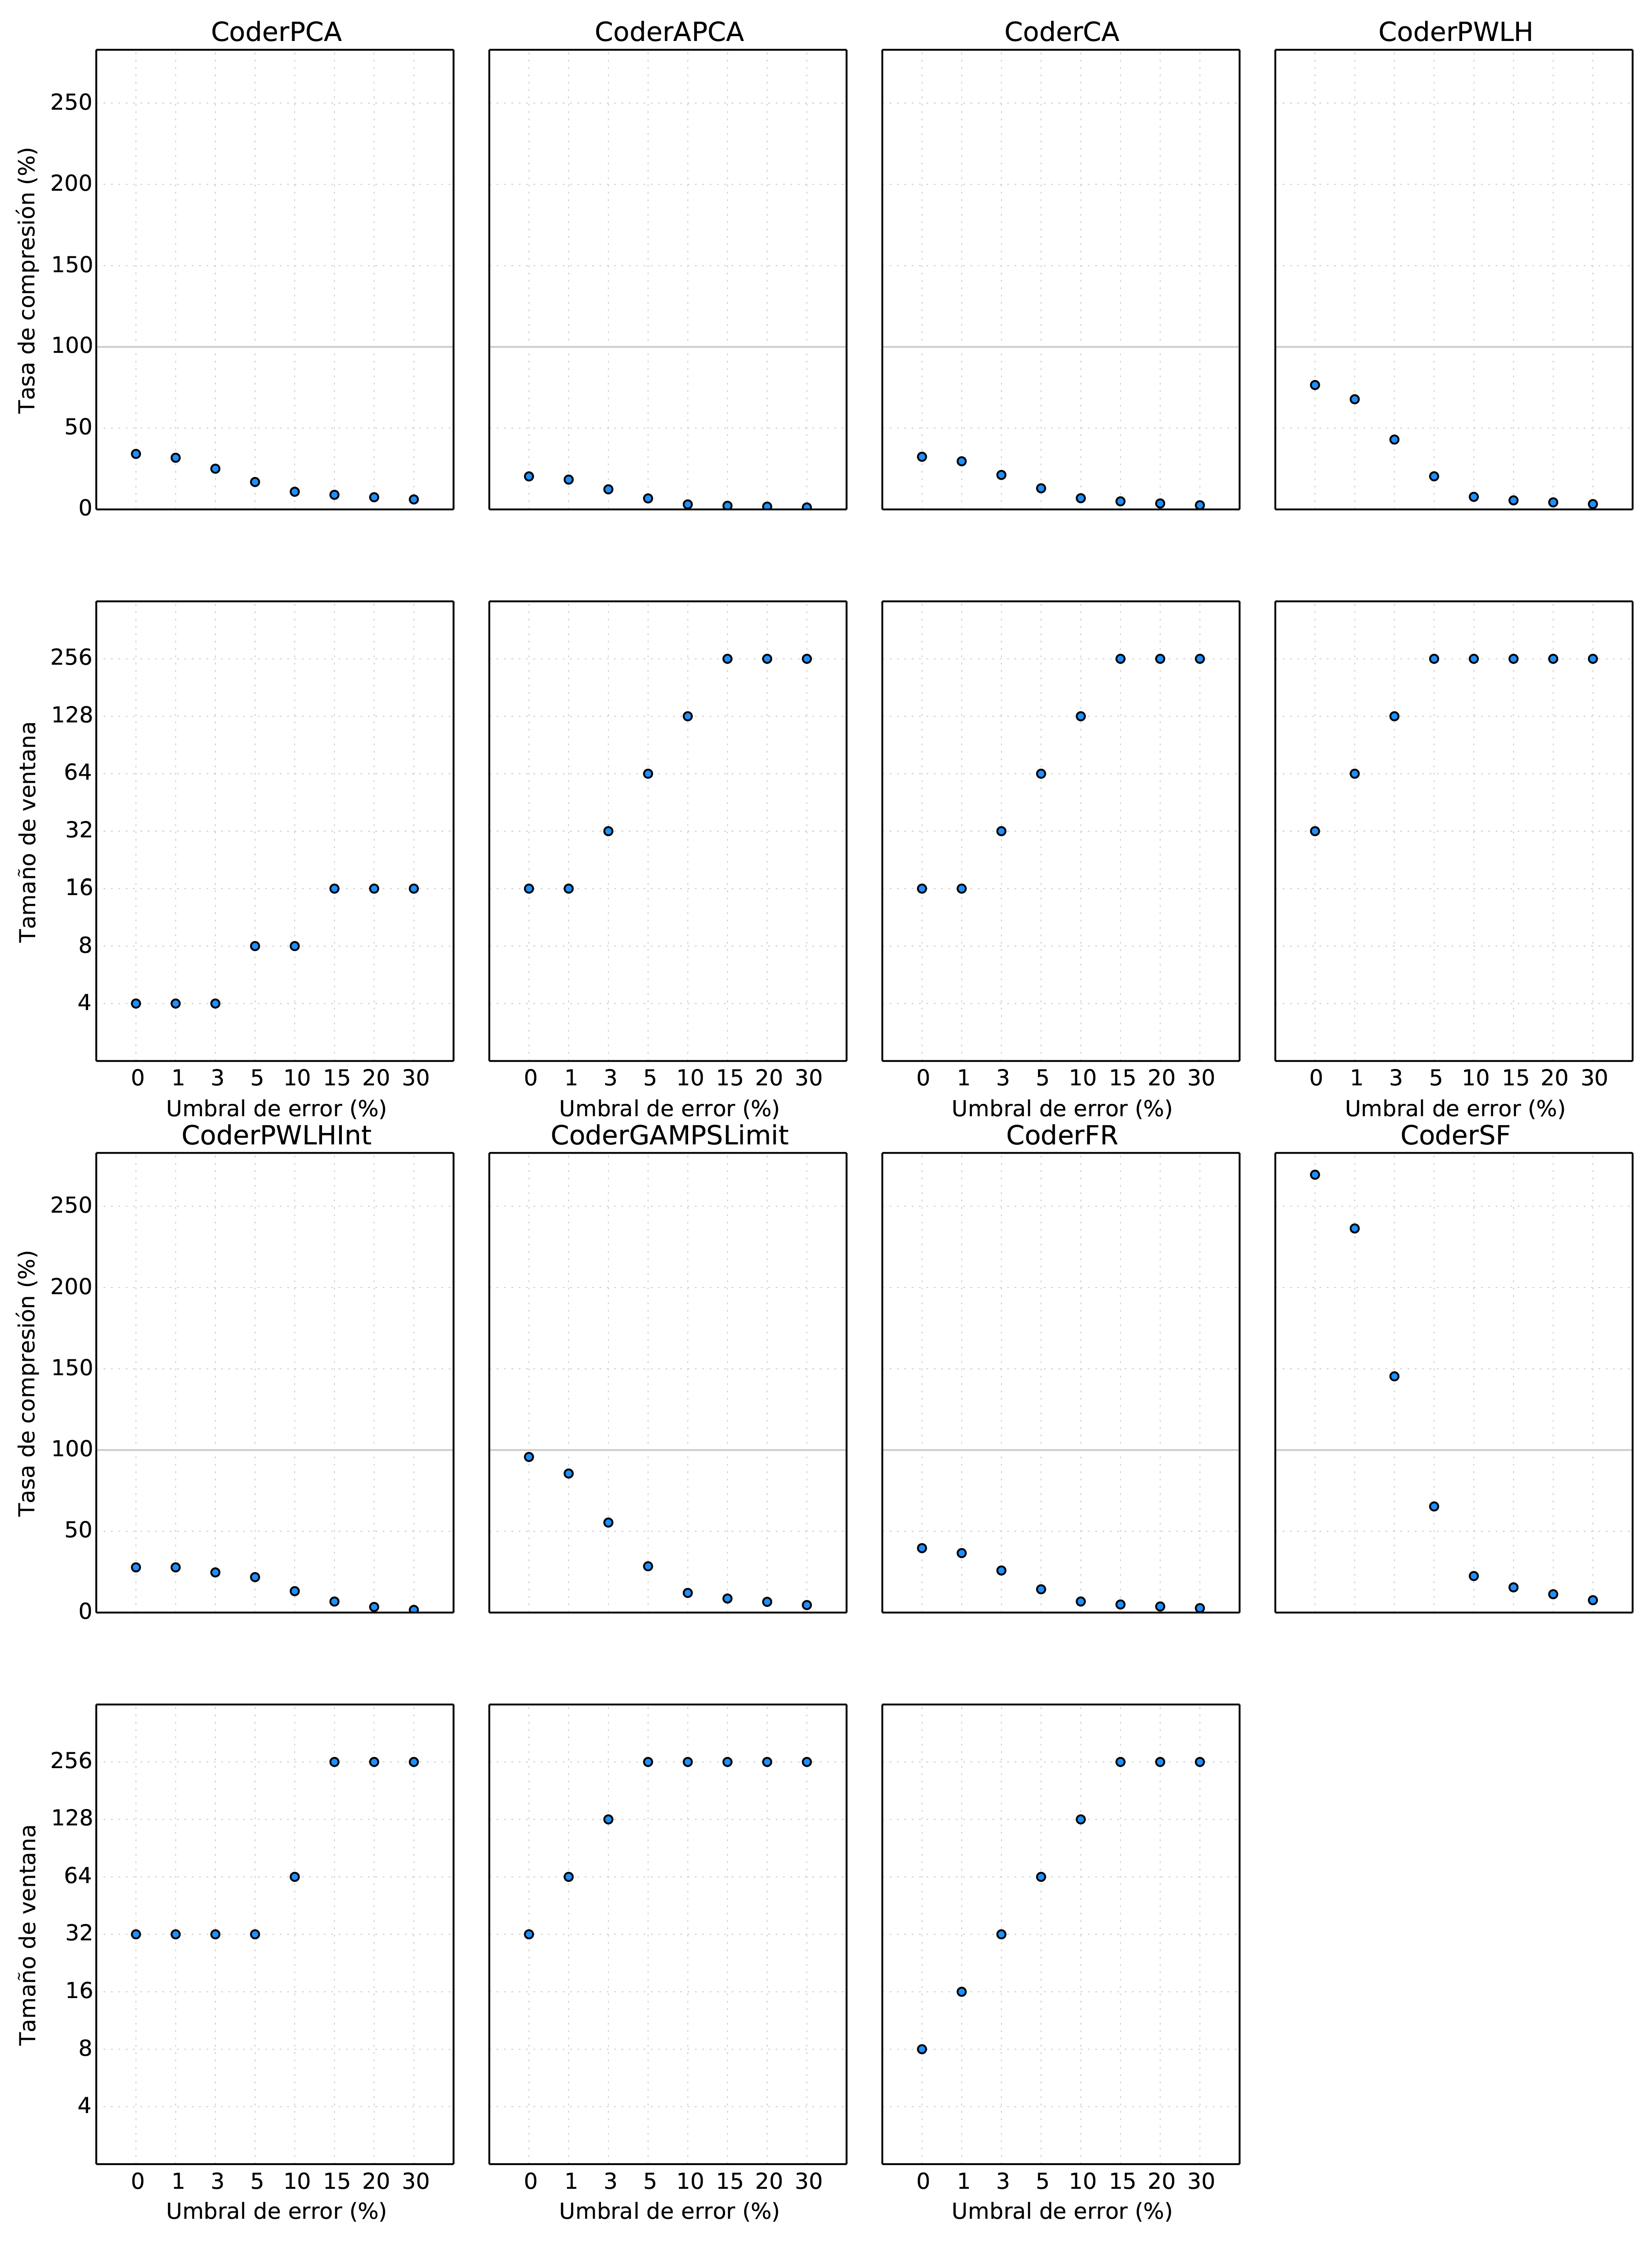
\includegraphics[scale=0.50]{chapters/Experiments/images/1-IRKIS.png}
\hspace{+10pt}
\caption{Compression rate and Window size graphs for the different combinations\\<$\coder \in C$, $w \in W, e \in E$> for the ``VWC" data type of the \datasetirkis \ dataset.}
\label{fig:mask-irkis}
\end{figure}

\clearpage







\clearpage
\section{Comparison with the gzip Algorithm}
\label{secX:gzip}